\documentclass{article}
\usepackage{polski}
\usepackage[utf8]{inputenc}
\usepackage{indentfirst}  
\usepackage[english]{babel}
\usepackage[left=2.5cm,right=2.5cm,top=2cm,bottom=2cm]{geometry}
\usepackage{graphicx}
\usepackage{listings}
\usepackage{xcolor}
\overfullrule=1mm
\definecolor{codegreen}{rgb}{0,0.6,0}
\definecolor{codegray}{rgb}{0.5,0.5,0.5}
\definecolor{codepurple}{rgb}{0.58,0,0.82}
\definecolor{backcolour}{rgb}{0.95,0.95,0.92}
\lstdefinestyle{mystyle}{
	backgroundcolor=\color{backcolour},   
	commentstyle=\color{codegreen},
	keywordstyle=\color{magenta},
	numberstyle=\tiny\color{codegray},
	stringstyle=\color{codepurple},
	basicstyle=\ttfamily\footnotesize,
	breakatwhitespace=false,         
	breaklines=true,                 
	captionpos=b,                    
	keepspaces=true,                 
	numbers=left,                    
	numbersep=5pt,                  
	showspaces=false,                
	showstringspaces=false,
	showtabs=false,                  
	tabsize=2
}
\lstset{style=mystyle}
\graphicspath{ {./assets/} }
\parindent=10ex




\begin{document} %---------------------------------------------------------------------------------------------------------------------% 

\centerline{\textbf{\Large Seminarium magisterskie}}
\vspace{10mm}
{\Large Wykorzystanie cyfrowej analizy obrazu w metodykach pracy z dziećmi w wieku przedszkolnym}

\vspace{10mm}
\centerline{\large Jakub Lebiedziński} 
\vspace{1mm}
\centerline{\normalsize {269096}} 
\vspace{5mm} 

\linespread{1.3} % interlinia dla dalszej zawartości dokumentu = 1.5
\large % wielkość czcionki dla dalszej zawartości dokumentu

\section*{Wstęp}

\par
Prawdopodobnie czytając te słowa w niedalekiej odległości kilku metrów od czytelnika znajdują się co najmniej trzy urządzenia elektroniczne podłączone do Internetu. Dzieje się tak, ponieważ obecny świat wymaga dostępu do małych komputerków z potężną mocą obliczeniową (porównując oczywiście do urządzeń sprzed kilku dekad), dzięki której nasze życie jest równie proste co skomplikowane. Dlaczego? Nie, nie dlatego, że nie potrafimy kupić elektronicznego biletu z aplikacji. Również nie dlatego, że momentami mamy wrażenie jakoby telefon był mądrzejszy od jego posiadacza i sam mówił mu co ma robić. Możliwości jakie dają nam urządzenia wykorzystujące dzisiejszą technologię przekraczają wszelkie wyobrażenie normalnego człowieka. Potęga mocy obliczeniowej i wielozadaniowości w jaką wyposażona jest niemalże każda maszyna, począwszy od kamery monitoringu, skończywszy na serwerowni wielkiej korporacji OVH zaopatrującą pół Europy w dostęp do sieci WWW, stawia przed nami wyzwanie. Wyzwaniem tym jest umiejętne jej wykorzystanie w celu poprawy i ułatwienia naszego życia jednocześnie balansując między prostotą a skomplikowaniem.
Celem niniejszej pracy magisterskiej będzie wskazanie na rosnącą rolę technologii cyfrowej w kontekście edukacji w ujęciu ogólnym. Praca podzielona jest na 4 rozdziały.
\par 
Pierwszy z nich jest wstępem do tematyki ogólnej edukacji dzieci z elementami wykorzystującymi pomoce dydaktyczne. Zwraca szczególną uwagę na postrzeganie świata przez dzieci i doświadczanie go za pomocą zmysłów. Czytając go przemierzamy tysiące lat, od starożytności po czasy nowożytne skupiając się na roli i potrzebie nauki. Poznajemy metody kształcenia, które w swoich czasach uważano za skuteczne, a także podważamy je porównując z dowodami lat późniejszych.
\par
W drugim rozdziale niniejszej pracy kładę większy nacisk na edukację w dwudziestym wieku i początek epoki przemysłowej, która niewątpliwie była początkiem rozwoju technologii informatycznej, o której mowa w poniższych rozważaniach.
\par
Trzeci rozdział poświęcam czysto technologicznym rozważaniom na tematy cyfrowej analizy i przetwarzania obrazów. Wskazuję wady i zalety niektórych rozwiązań. Rozbijam na czynniki pierwsze prototypy fotografii cyfrowej i analizuje sposób działania analogowych urządzeń do uwieczniania świata na “kawałku taśmy”.
\par
Czwarty i ostateczny rozdział opisuje najświeższe rozwiązania współczesnej techniki wykorzystujące obraz jako kontener z danymi do analizy i implementacji różnego rodzaju algorytmów. Dodatkowo zawiera moje przypuszczenia i przewidywania kierunku, w którym zmierza dzisiejsza technologia w kontekście cyfrowej analizy i przetwarzania obrazów.
\par
Całość pracy jest okraszona fotografiami schematów, porównań, fragmentami oprogramowania stworzonego na potrzeby badań oraz bibliografią, na podstawie której zebrałem informacje do napisania poniższej pracy.

\section{Historia edukacji w pojęciu nauczania najmłodszych}
\subsection{Edukacja kiedyś a edukacja dziś}

\par
Edukacja jest z nami od zarania dziejów. Już w starożytnej Grecji powstawały pierwsze ‘szkoły’, gdzie słuchacze mogli śledzić wykłady najznamienitszych filozofów ówczesnego świata. Platon, Arystoteles czy Sokrates byli uważani za mistrzów retoryki, etyki czy filozofii. Warto wspomnieć, że nie każdy obywatel antycznego państwa miał obowiązek pobierania nauki. Edukacja była bowiem przywilejem, na który stać było tylko najbogatszych. Dzisiaj jest to nie do pomyślenia. Z czasem jednak edukacja stawała się coraz bardziej dostępna dla niższych warstw społecznych. Dawni nauczyciele wspomagali się w edukowaniu swoich słuchaczy wskaźnikami, elementami natury, mapami, malunkami i tak dalej. Podobnie jest i teraz. Różnicą jest stopień zaawansowania ‘pomagaczy’ i procent ich wykorzystania w szkolnictwie.
\par
Nie sposób napisać ile się zmieniło przez tysiące lat, ale jedno jest pewne - jak napisał \cite{ref1} Marcin Bojarski w swoim felietonie “Przekazywanie wiedzy młodszym przez osoby doświadczone jest najpewniej procesem tak starym jak człowiek”. Trudno się nie zgodzić. Od momentu poczęcia, jeszcze zanim ujrzymy świat, w naszym zachowaniu da się dostrzec pewne schematy wyuczone przez te kilka miesięcy etapu płodowego, który trwa między jedenastym, a czterdziestym tygodniem okresu prenatalnego.
\par
Nie będę cofał się aż do czasów Adama i Ewy, ale postaram się zacząć od spojrzenia na edukacja w czasach antycznych. Do czasu wynalezienia pisma starsi przekazywali swoje mądrości w sposób werbalny i wymagający zapamiętania dla przyszłych pokoleń. Jakże wielkim wynalazkiem było wynalezienie pisma i zdjęcie obowiązku z człowieka z zapamiętywania wszystkiego co mówił dziadek - niech żyje pismo! Od tego momentu edukacja jako przekazywanie wiedzy nabrała tempa. W starożytnym Egipcie i Mezopotamii wybrańcami, którzy posiedli umiejętność zapisywania i czytania była kasta skrybów, którzy służyli władcy i jego rodzinie. W głównej mierze uczono matematyki, ale też czytania i pisania, co wówczas nie należało do podstawowych umiejętności dorosłego człowieka. Swoistym testamentem tamtych czasów są zachowane, nierzadko w idealnym stanie, hieroglify i kamienne płyty z wyrzeźbionymi symbolami, bądź rzadziej literami alfabetu. Początki nie zawsze były kolorowe. Zanim pozwolono młodym uczniom na samodzielne zapiski na papirusie musieli oni uprzednio posiąść fach w pisaniu na tak zwanych ostrakach czyli glinianych tabliczkach.
\par
Odmienny stan rzeczy, według obecnej wiedzy naukowców, miał miejsce we wschodniej Azji, a dokładniej w Chinach. Ówczesnymi osiągnięciami chińskiej nauki był niesamowity rozwój medycyny co skutkowało wynalezieniem akupunktury, akupresury czy moksy. Dostęp do nauki był znacznie szerszy niż we wspomnianym Egipcie i nie dotyczył tylko władcy oraz jego najbliższego otoczenia. Zachowały się informacje mówiące o tym, że już w czasach dynastii Zhou (lata 1045 - 256 przed naszą erą) dość powszechne były szkoły dla najmłodszych. Początkowo uczono w nich, zależnie od płci, praktycznych rzeczy, które przydadzą im się w dalszym życiu. Nauki te nosiły nazwę “Sześć sztuk” i składały się na nie wiedza o matematyce, kaligrafii, muzyce czy łucznictwie. Z drugiej strony płeć piękna szlifowała fach w tkactwie, hafcie czy jedwabnictwie. Również w astronomii chińscy uczeni udowodnili swoje umiejętności dokładnie opisując zjawiska zachodzące w przestrzeni kosmicznej. Mowa tu o zaćmieniach Słońca czy Księżyca, opisami gwiazdozbiorów czy układem gwiazd na niebie. To ostatnie było bardzo ważne, bowiem wierzyli oni, że ułożenie gwiazd nie jest przypadkowe i w zależności od ich pozycji może zwiastować przepych i dobrobyt albo zgubę i zagładę. Wszystko w kontekście panującego władcy. Nie muszę dodawać jak oddanym narodem są Chińczycy. Ich ciężka praca i lojalność są nieocenione i skutkowały wynalezieniem, a z czasem zrewolucjonizowaniem ówczesnej gospodarki, czterech najważniejszych wynalazków. Są to kolejno papier, proch, kompas oraz druk. Tysiące lat później większości z nich wciąż używa się na co dzień, choć w zmienionej formie to nie można zapominać kto był prekursorem do ich wynalezienia.
\par
Kolejnymi cywilizacjami, które niejako dopełniają obraz starożytnej nauki są Cesarstwo Rzymskie i Grecja. W pierwszej z nich wyróżnia się dwa etapy kształcenia świadomości dziecka - granica jaka rozgranicza niejako te dwa etapy jest wiek siedmiu lat. Do tego czasu za wychowanie moralne zarówno córki jak i syna odpowiadała wyłącznie ich matka. Z kolei tuż po osiągnięciu wyżej wymienionego wieku synowie przechodzili pod opiekę drugiego rodzica - ojca, który miał zadbać o edukację i wykształcenie syna z zakresu wojskowości i wiedzy ogólnej niezbędnej w życiu prywatnym. Na te drugie składały się: umiejętność pracy na roli, podstawy zarządzania zasobami ludzkimi w kontekście nadzoru nad służbą i niewolnikami, a także elementy rzemiosła połączone z wykorzystaniem narzędzi do celów obronnych w zakresie wojskowości. Lwią część wiedzy rzymskie dzieci nabywały na wolnym powietrzu wraz ze swoimi rówieśnikami wspólnie biorąc udział w grach terenowych mających na celu przygotowanie młodych do trudów związanych z warunkami panującymi na terenie działań wojennych. Do gier i zabaw, które sprzyjały rozwojowi i świadomości młodych Rzymian należały między innymi jazda konna, umiejętność posługiwania się bronią czy elementy musztry i kamuflażu w trudnym terenie.

\subsection{Współczesny nauczyciel}

Nie sposób opisać jak na przestrzeni wieków zmieniała się rola nauczyciela w społe-czeństwie. Począwszy od roli przez formę wykonywania zawodu na samej nazwie “nauczyciel” kończąc. Można powiedzieć, że to dwa różne zawody, które docelowo miały zbliżone obowiązki - przekazać swoją wiedzę innemu człowiekowi. Co więcej, Jarosław Rudziński uważa, że “we współczesnej epoce wychowanie odgrywa lub odgrywać powinno rolę najważniejszą, a zawód nauczyciela jest w rzeczywistości najważniejszym, ze wszystkich obecnie istniejących”. Zapewne wiele osób nie zgodziłoby się z tymi słowami, natomiast jedno jest pewne - edukacja młodych ma ogromny wpływ na kształtujące się społeczeństwo (które de facto będzie w niedalekiej przyszłości składało się z obecnie bardzo młodych ludzi). Współczesnemu nauczycielowi, według mojej opinii, nie okazuje się szacunku na jaki zasługują - zarówno ze strony młodych jak i tych nieco starszych. Wielokrotnie bywałem świadkiem kuriozalnych sytuacji, w której rola nauczyciela była marginalizowana do minimum, a jego zdanie było bagatelizowane i czasami w ogóle nie brane pod uwagę. Często nie zdajemy sobie sprawy, że bez odpowiedniego podejścia już na samym początku niechęć do edukatora z czasem się pogłębia i dochodzimy do wyżej opisanego momentu. Warto mieć na uwadze, że im młodszy uczeń tym rzadziej powinien otrzymywać lekcje od nauczyciela - dlatego w edukacji wczesnoszkolnej i przedszkolnej nauczyciele obejmują jeden rocznik i przechodzą z nim przez 3 lata (czasami dłużej) do momentu, w którym dziecko osiąga taki stopień świadomości na oddzielenie się od swojego wychowawcy i jest gotowe do rozpoczęcia pobierania nauki u innej osoby.

\subsection{Edukacja dzieci w wieku przedszkolnym}

\par
W tym podrozdziale skupię się na dzieciach w wieku przedszkolnym, ponieważ od najmłodszych lat można dostrzec schematy i utrwalanie pewnych zachowań w nauce podstawowych czynności takich jaki mówienie, pisanie czy postrzeganie świata. Józef Bednarek w swojej książce pod tytułem ‘Multimedia w kształceniu’, iż każdy uczeń chce się uczyć, ale to podejście pedagoga jest niezbędnym elementem, aby ta nauka ‘nie poszła w las’. Porównanie ww. autora, tablicy i kredy do telewizji i gier komputerowych wydaje się trafnym porównaniem podkreślającym rolę jaką odgrywa współczesny nauczyciel. Z pomocą przychodzi już wspomniana technologia. 
\par
Dzieci w wieku przedszkolnym tj. 3-6 lat są niezwykle wrażliwe na bodźce ze świata zewnętrznego. Przy oglądaniu zdjęć, obrazów, malunków ich mózg skupia się na rozpoznawaniu kształtów, kolorów, osób, a z wiekiem potrafi zauważyć analogię pewnych zestawień liter, kolorów, a nierzadko jest w stanie je nazywać. W swojej pracy wykorzystuje autorskie rozwiązanie interaktywnej kolorowanki w czasie rzeczywistym. Ów narzędzie opiera się na rozpoznawaniu kolorów, rysowaniu kształtów oraz stymuluje prawidłowy rozwój dziecka w myśl zasady - nauka poprzez zabawę. Zakresem badań będą przeprowadzenie serii eksperymentów i zapis obserwacji oraz wnioski z zachowań dzieci bawiących się wyżej opisanym narzędziem.
\par
Wracając do rozwoju dziecka w wieku przedszkolnym nie sposób zauważyć, że ten trzyletni okres jest na tyle ważny dla poprawnego zrozumienia świata, które dopiero co to dziecko poznało, że należy go podzielić na pewne etapy. Spotkałem się z podziałem na cztery etapy, ale skupię się na pierwszych trzech, gdyż uważam je za fundamentalne i kluczowe we właściwym procesie odbioru bodźców wysyłanych przez ten świat.
\par
Pierwsza faza jest typowo wrażliwa i cechuje się brakiem dostosowania się dziecka do otoczenia. Ma ono problemy ze zmianami zachodzącymi w jego życiu. Naturalnie w tej fazie dziecko jest najmniej samodzielne i wymaga ciągłej pomocy w podstawowych czynnościach.
Faza druga to tak zwana. “faza pytań”. Dziecko nieustannie zadaje odpowiedzi czym zaznacza rozwój świadomości istnienia i coraz częściej potrafi samodzielnie wykonać rzeczy, których nie potrafiło w fazie pierwszej. W tej fazie najbardziej zauważalny jest postęp w mowie i rozwoju myślenia dziecka. Dodatkowym atutem dla rodziców (choć nie zawsze) jest wyraźne zaciekawienie dziecka elementami otoczenia czyli innymi słowy poszerzana jest przez dziecko wiedza o swoich zmysłach takich jak dotyk czy węch.
\par
Trzecia faza rozwoju dziecka w wieku przedszkolnym naznaczona jest drobnymi poleceniami do wykonania przez dziecko. Coraz śmielej podejmuje ono inicjatywę w niesieniu pomocy dorosłym, jest na tyle samodzielne, że nie wymaga ciągłego nadzoru dorosłego. Chętnie bierze udział w grach i zabawach, nie ma problemu z nawiązywaniem kontaktu z rówieśnikami. W tej fazie dziecko jest w stanie skoncentrować swoją uwagę na dłużej i nie stanowi to dla niego dużego problemu.
\par
Ostatnia faza to okres dziecka od około 5 do 7 lat, dlatego przyjęło się, że wówczas jest ono gotowe na podjęcie edukacji w szkole podstawowej. Dziecko jest na tyle samodzielne i potrafi rozwiązywać proste problemy, że jest w stanie słuchać poleceń nauczyciela i wspólnie pracować w grupie innym dzieci. Niewątpliwie bardzo dużo zależy od tego jak przebiegały wszystkie trzy fazy rozwoju dziecka. Czy miało ono wystarczająco dużo czasu na poprawne zinterpretowanie bodźców, czy jego rozwój stymulowany był w odpowiedni sposób przez rodziców. Zdarza się, że dziecko nie nadąża nad zmianami i potrafi “utknąć”, w którejś z trzech faz dlatego tak ważna jest obserwacja i pomaganie dzieciom w uczeniu się pewnych zachowań. Z pomocą przychodzą gry dydaktyczne, kolorowanki, a we wcześniejszych fazach zabawki sensoryczne pozwalające dziecku poznać siebie i swoje zmysły.



\section{Multimedia w szkolnictwie}
Z biegiem lat zauważamy coraz to nowsze rozwiązania technologiczne wprowadzane począ- wszy od szkół podstawowych, a skończywszy do szkolnictwie wyższym. Kiedyś hitem były tablice multimedialne, które stawały się niemalże wizytówką placówki oświatowej. Tak było kilka lat temu. Rok 2020 okazał się jeszcze bardziej wymagający i zmusił szkoły, organy oświatowe a także samorządy i placówki administracyjne do zakupu wszelkiego rodzaju tabletów, laptopów, notebooków, smartfonów etc. Nagle okazało się, że podstawowy ekwipunek ucznia o wadze 11 kilogramów został zastąpiony jednym 800g tabletem, w którym znajdują się elektroniczne wersje niezbędnych do nauki podręczników i ćwiczeń. W przedszkolach również zauważa się wzrost technologii wykorzystywanej do nauki dzieci. Co prawda komputery już wcześniej były obecne w salach zabaw, a dzieci potrafiły w mniej lub bardziej logiczny sposób wyjaśnić obecność elektroniki, ale elektroniczna kolorowana to coś całkiem nowego dla całego półświatka przedszkolnego. 
\section{Język C++}
Zapewne każdy aspirujący programista musiał miał styczność z tym językiem. Prosty, niewy- magający, wybaczający błędy - idealny do rozpoczęcia przygody z programowaniem. Język C++ to nie jest “związek” tylko na chwile. Jego zastosowanie można zaobserwować w takich produktach jak Windows, Mac OS, pakiet Adobe czy Office. Dlaczego? Odpowiedź jest prosta - język C++ jest bardzo wydajny i zużywa o wiele mniej zasobów przy kompilacji. Jak słusznie zauważa Karol Kuczmarski w swojej książce “Kurs C++. Od zera do gier kodera” \cite{ref5} mocnym atutem języka C++ jest jego popularność i dostępność rozwiązań. Cytując jego słowa można stwierdzić, że “[...] C++ zdaje się być bardziej uniwersalny (od języka Delphi, przyp. tłum.). Dobrze rozumie się z ważnymi dla nas bibliotekami graficznymi, jest także bardzo szybki i posiada duże możliwości” Jak to się stało, że język C++ osiągnął taką przewagę nad innymi językami? Żeby odpowiedzieć na to pytanie należy cofnąć się do początków lat siedemdziesiątych kiedy to niejaki Dennis Ritchie finalnie zaimplementował z pomocą języka C jądro systemu operacyjnego Unix. Uznaje się to wydarzenie za początek dominacji języka C (i jego późniejszych ewolucji, o których 
wspomnę w dalszej części). Po roku 1980 język C (a także jego późniejsza wersja z dwoma plusami) wiódł prym w programowaniu systemów i aplikacji czego dowodem był produkt Microsoftu pod nazwą Windows, przy którego budowanie w znacznej mierze opierano się na wyżej wymienionym języku programowania. Warto zaznaczyć, że język C/C++ posiadał bardzo ważną cechę jaką niewątpliwie jest możliwość przenoszenia go na inne urządzenia. Dodatkowym atutem, o którym trzeba powiedzieć jest to, że większość dzisiejszych sterowników do kart graficznych, dźwiękowych i tak dalej są pisanie niskopoziomowo z wykorzystaniem właśnie języka C/C++.
\section*{\textbf{Ewolucji ciąg dalszy czyli język C Sharp}}
W końcówce lat dziewięćdziesiątych zaczęto zastanawiać się na stworzeniem od podstaw języka programowania opartego na obiektowości, który mógłby rywalizować z zyskującą popularność Javą. Narodził się pomysł utworzenia zespołu projektowego, którego zadaniem byłoby stworzenie mocnego konkurenta na “rynku obiektowości” w myśl zasady głoszonej przez model PME (Properties - Methods - Events). Na czele projektu stanął charyzmatyczny Duńczyk Anders Hejlsberg - znany i ceniony programista w środowisku informatycznym. W swoim dorobku miał doświadczenie w pracy nad takimi językami jak wspomniany już wcześniej Delphi, Pascal, a później również TypeScript. W swojej książce pod tytułem “The C\# Programming Language” \cite{ref6} wspominał, że praca przy nowym języku była dla niego nie lada wyzwaniem, ale zaznaczył, że traktował to jako ciekawą rozrywkę, żeby nie powiedzieć zabawę. Dodał, że miarą rozwiązywania problemów jest dodanie wartości tworzonemu produktowi przy poszukiwaniu solucji.
\section*{\textbf{Programowanie GPU}}
Jak wspomniałem jedną z zalet języka C/C++ jest szeroki zasób i dostępność do bibliotek o bardzo różnym charakterze. Od napisania mikrokontrolera przez fotokomórkę aż po grę komputerową. W dzisiejszym świecie coraz więcej elementów otaczającego nas świata zależy właśnie od technologii. Częściej musimy zasięgnąć opinii przysłowiowych “informatyków”, aby Ci wytłumaczyli nam chociażby jak kupić bilet na autobus z poziomu telefonu komórko- \ wego. Wraz z rozwojem sektora oprogramowania graficznego na znaczeniu, w kwestii mocy obliczenio- \ wej, zyskały układy graficzne oparte głównie na dwóch architekturach - NVIDIA CUDA oraz OpenCL. Zauważono, że obecnie układy te pozwalają na wykonanie serii bardziej skomplikowanych operacji niż dotychczas sądzono. Nowoczesne procesory graficzne są w stanie generować żądany obraz w czasie rzeczywistym i co więcej są w stanie zmodyfikować go według określonych zasad ustanowionych przez programistę. Dzieje się tak, gdyż układ CPU komunikuje się z układem GPU z pomocą specjalnego API (Application Programming Interface) w charakterze komunikatora pomiędzy dwoma układami. Poniższy schemat powinien nieco rozjaśnić powyższe rozważania.
\begin{center}
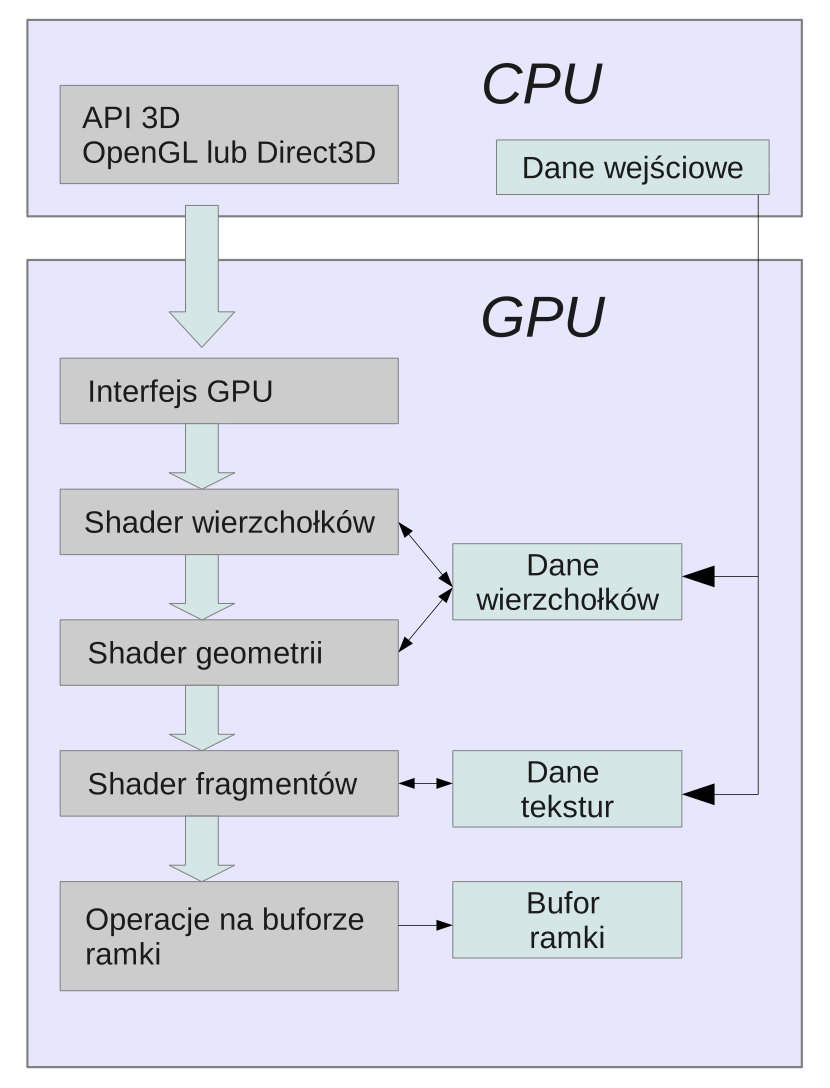
\includegraphics[width=10cm]{gpu}
\end{center}
Dzięki takiemu rozwiązaniu powszechne stało się wykorzystanie mocy obliczeniowej procesorów graficznych w tworzeniu oprogramowania wykorzystującego funkcje przetwarzania obrazu przechwyconego z kamery. Przykładem takiego rozwiązania jest na przykład rozpoznawanie twarzy w nowoczesnych telefonach, skanowanie numerów rejestracyjnych samocho- dów wyjeżdżających z parkingów, algorytmy rozpoznawania elementów na obrazie w celu identyfikacji i opisania rzeczy znajdujących się przed obiektywem kamery. W nowych samochodach można znaleźć system odpowiadające za śledzenie toru, po którym porusza się pojazd, albo oprogramowanie odpowiadające za detekcję znaków drogowych i stosowanie odpowiednich ograniczeń wbudowanych w oprogramowanie komputera pokładowego. Można by wymieniać i wymieniać, ale żeby “namacalnie” (a przynajmniej w teorii) móc poczuć wcześniej wspomniany skok technologiczny warto chociażby zdobyć i porównać zdjęcia dwóch gier wideo, których daty premier oddalone są na osi czasu o raptem 20 lat. W ciągu tak krótkiego czasu zrobiono więcej niż przez ostatnie 50 lat w kwestii motoryzacji (chociaż Elon Musk każe sądzić inaczej). Jestem bardzo ciekaw jak będzie wyglądać rozgrywka za drugie tyle lat. Prawdopodobnie niemożliwym zadaniem będzie odróżnienie gry od rzeczywistości.
Sekretem realistycznej grafiki w grach komputerowych jest skomplikowanie algorytmów odpowiedzialnych za renderowanie w czasie rzeczywistym tekstur w bardzo wysokiej rozdzielczości. Swoim artykule Christoph Liedtke z redakcji GameStar (gamestar.de) \cite{ref7} zwraca szczególną uwagę na nowe efekty graficzne, które pojawiły się wraz z rozwojem mocy obliczeniowej kart graficznych “Również efekty graficzne takie jak np. mapowanie wypukłości (bump mapping), multiteksturowanie czy też oparta na rzeczywistych obrazach technika fotogrametrii, a także pakiety tekstur o wysokiej jakości tworzone przez fanów, sprawiają że pod względem graficznym gry stają się coraz bardziej imponujące.”\\
\begin{center}
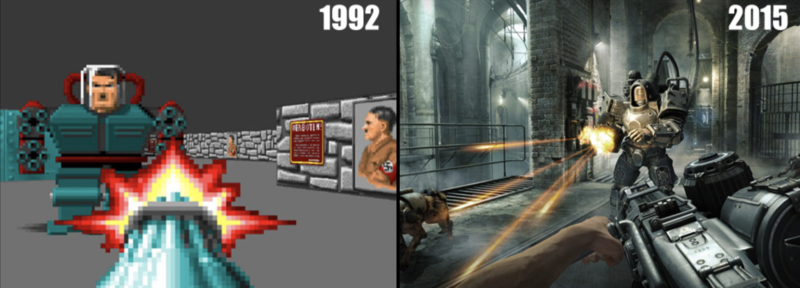
\includegraphics{grafika}
\end{center}
\section*{\textbf{Cyfrowa analiza obrazu}}
Aby wyjaśnić sposób działania algorytmów odpowiedzialnych za analizę fotografii czy obrazu z aparatu/kamery trzeba nieco cofnąć się w czasie do klasycznej fotografii.
W czasach, gdy ludzie chcieli upamiętnić ważną chwilę trudno szukać jako takiej technologii znanej nam dzisiaj. Czy można powiedzieć, że wraz z rozwojem fotografii cyfrowej, wymyślono aparat na nowo?. O tym za chwilę. Na ten moment zostańmy jeszcze chwilę w tematach, jak to się dziś ładnie mówi - retro. Klasyczne, żeby nie powiedzieć stare, aparaty fotograficzne działają w oparciu o nośniki wykorzystujące materiały światłoczułe (np. klisze). Trzeba zaznaczyć, że klasyczny nie jest równy analogowy. W rozumieniu analogowy mamy na myśli te, które nie wykorzystują sygnału cyfrowego do zapisu obrazu na materiale światłoczułym. Błędne określenie aparatów analogowych klasycznymi pojawiło się wraz z rozwojem fotografii cyfrowej. Trzeba z tego zapamiętać tyle, że w dawnych aparatach klasycznych nie stosowano zapisu obrazu za pomocą sygnału analogowego. Tymczasem świat poszedł naprzód, a to co najważniejsze, ludzie zaczęli “zapamiętywać” swoje życie na cyfrowych matrycach nowoczesnych aparatów. Cyfrowy zapis od analogowego różni się tym, że w tym pierwszym fotografia utrwalana jest binarnie na matrycach cyfrowych, które po błyskawicznym “przetłumaczeniu” oddaje obraz w różnych barwach reprezentowanych przez ciąg zero-jedynkowy. Każdy taki obraz składa się z setek, tysięcy pikseli. Każdemu pikselowi odpowiada konkretny obszar i zapis na ww. cyfrowej matrycy. Innymi słowy, działanie aparatu takie same, ale zapis już niekoniecznie. Mając zapis binarny zdjęcia możemy dzięki algorytmom zastosować szereg operacji mających na celu np. rozpoznanie tekstu, detekcję ruchu, zliczanie elementów czy wspomnianą już wcześniej asystę dla kierowcy przy zjeździe z pasa na jezdni. Maszyna mając zero-jedynkowe przedstawienie fotografii widzi macierz liczb, która zawiera reprezentację barw.
\begin{center}
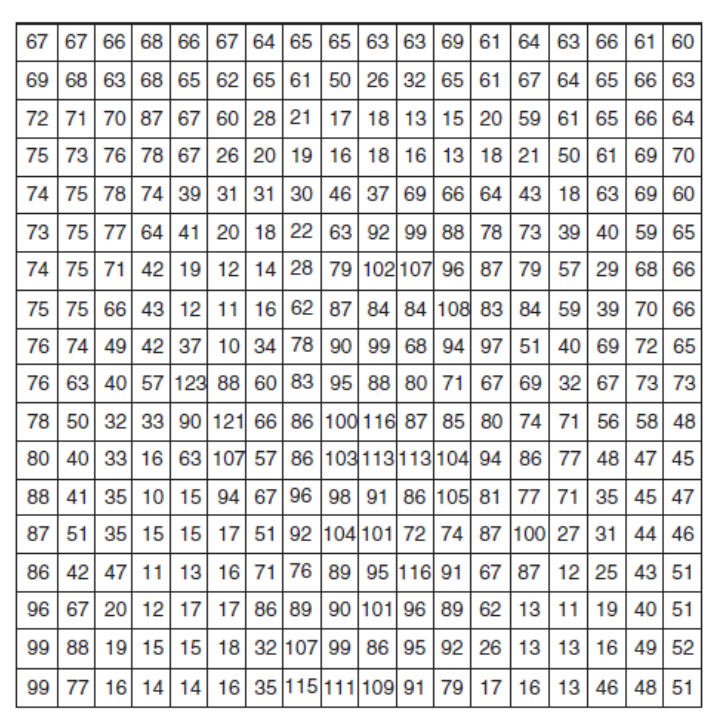
\includegraphics[width=10cm]{macierz}
\end{center}
Jest to jedna ze struktur obrazów cyfrowych, które “rozumie” maszyna. W głębszym rozumieniu, pozyskiwanie obrazów cyfrowych i translację ich na język komputerowy nazywamy dyskretyzacją obrazu. Ryszard Tadeusiewicz i Przemysław Korohoda w “Komputerowej analizie i przetwarzanie obrazów” \cite{ref8} zaznaczają, że ów sztuczna reprezentacja i sposób jej kreowania posiada swoje ograniczenia wynikające z wydajności dzisiejszych maszyn. Niestety (a może i stety) nie osiągnęliśmy jeszcze poziomu maszyn, które można byłoby określić szybszymi i mądrzejszymi niż zmysły ludzkie (w tym wypadku mam na myśli zmysł wzroku). Na ten moment uważa się, że przybliżone przetwarzanie danych w czasie rzeczywistym przez ludzkie oko plasuje się na poziomie około stu megabajtów na sekundę co przekracza możliwości komputerów w znanym nam świecie. Być może, a raczej wielce prawdopodobne, jest to, że maszyna oparta o technologię kwantową sprostałaby wyżej wymienionym wymaganiom, ale na tę chwilę musimy te rewelacje odsunąć na bok i skupić się nad dostępnością dzisiejszych rozwiązań. Co możemy zrobić, aby ograniczyć reprezentację obrazu? Ryszard Tadeusiewicz i Przemysław Korohoda wymieniają między innymi możliwość ograniczenia fotografii poprzez zmniejszenie ilości szczegółów, ale też uproszczenie i ujednolicenie stanów elementów (na przykład poprzez wykorzystanie czarno-białej palety barw). Autorzy sugerują również analizowanie obrazu płaskiego zamiast przestrzennego i statycznego zamiast dynamicznego. Ten ostatni przypadek odnosi się do ciągu klatek (obrazów) dlatego w dalszej części nie będę go brał pod uwagę. Warto mieć to jednak na uwadze. Dzisiejsze algorytmy przetwarzające fotografie wykorzystują jeden z dwóch sposobów umieszczenia cyfrowych odpowiedników elementów obrazu (pikseli). Są to: heksagonalne i kwadratowe.
\begin{center}
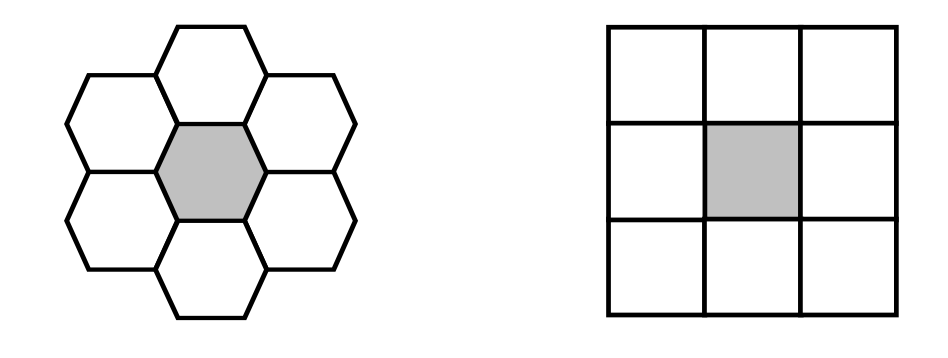
\includegraphics[width=15cm]{dyskretyzacja}
\end{center}
Wspomniana macierz reprezentująca barwy, a dokładniej nasycenie jednej z trzech bar modelu RGB (Red - Green - Blue), służy komputerowi jako źródło kilku istotnych danych. Maszyna rozpoznaje nasycenie, barwę oraz potrafi rozpoznać co znajduje się na pierwszym, drugim planie i tak dalej. Niemniej jednak to wciąż za mało, aby być pewnym otrzymanych wyników. Na dane wejściowe nierzadko stosuje się szereg zabiegów mających na celu zniwelowanie niedoskonałości powstałych przy wykonywaniu fotografii.
Zanim jednak zajmiemy się wyżej wymienionymi operacjami należy sobie wyjaśnić z czego biorą się błędny przy pracy ze źle przygotowanymi danymi wejściowymi. Niestety czynnik ludzki ma tutaj ogromne znaczenie dla wysokiej wartości tych danych. Często nie przywiązujemy należytej uwagi do jakości aparatów i ich podzespołów co prowadzi od początku do niewystarczającej ostrości, naświetlenia i tym podobne. Również pośpiech nie jest dobrym doradcą w tych sprawach. Ważną cechą dobrego zdjęcia jest odpowiednie światło i ostrość - co w przypadku obiektów poruszających się jest niezwykle utrudnione, żeby nie powiedzieć niemożliwe. 
\section*{\textbf{Operacje na fotografiach}}
Usuwanie szumu z fotografii nie jest czymś nowym. Zasada działania algorytmów “odszumiających” jest całkiem prosta w wytłumaczeniu. Jak wcześniej wspomniałem, komputer widzi obraz jako macierz z setkami małych punktów (pikselami). Filtr odpowiedzialny za usuwanie szumu sprawdza każdy element fotografii i jej bliskie sąsiedztwo analizując wartości pikseli. Założeniem jest to, że każdy punkt o przybliżonej barwie, naświetleniu powinien mieć podobne wartości, a każde odchylenie od tej reguły traktowane jest jako niepożądane zachowanie i modyfikowane w zależności od parametrów “dobrych pikseli”. Metody usuwania szumu są dwie - poprzez średnią arytmetyczną i medianę. W przypadku pierwszej filtr nadpisuje analizowany obszar wartościami średnimi obliczonymi na podstawie barwy i ostrości. W drugiej metodzie piksel otrzymuję medianę z otaczającego go sąsiedztwa co czyni obraz bardziej wyrazistym, ale może powodować skrzywienia i wpływać negatywnie na geometrię obrazu.
\begin{center}
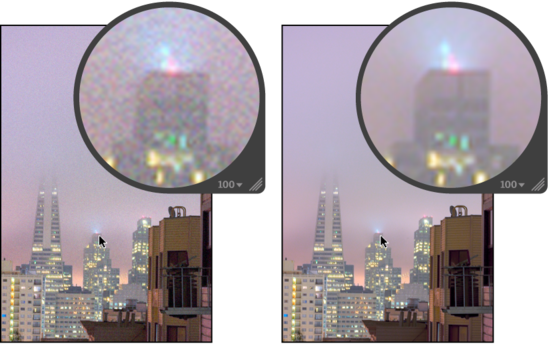
\includegraphics[width=15cm]{szum}
\end{center}
\newpage
\begin{lstlisting}[language=C++, caption=Początek wywołania]
	VideoCapture cap(0);
	
	//sprawdzenie dostepu do kamery urzadzenia
	if ( !cap.isOpened() )
	{
		cout << "Cannot open the web cam" << endl;
		return -1;
	}
	
	//uruchomienie okna z przechwyconym obrazem z kamery
	namedWindow("Control", WINDOW_AUTOSIZE);
\end{lstlisting}

Powyższy fragment kodu jest pierwszymi linijkami głównej metody wywołującej o nazwie main. Na początku sprawdzam czy mamy dostęp do kamery urządzenia. Następnie tworzę okno o automatycznych rozmiarach (skalowane w zależności od ustawień komputera, na którym uruchamiany jest kod).

\begin{lstlisting}[language=C++, caption=Klawisze funkcyjne]
	if (dArea > 10000) {
		int posX = dM10 / dArea;
		int posY = dM01 / dArea;        
		
		if (iLastX >= 0 && iLastY >= 0 && posX >= 0 && posY >= 0) {
			if (waitKey(60) == 113) {
				line(imgLines, Point(posX, posY), Point(iLastX, iLastY), Scalar(0,0,255), 15);
			}
			if (waitKey(60) == 119) {
				line(imgLines, Point(posX, posY), Point(iLastX, iLastY), Scalar(0,255,0), 15); 
			}
			else if (waitKey(60) == 101)
			{
				line(imgLines, Point(posX, posY), Point(iLastX, iLastY), Scalar(0,0,0), 15); 
			}
		}
		iLastX = posX;
		iLastY = posY;
	}
\end{lstlisting}

Powyżej zaimplementowane jest reagowanie programu na naciśnięte klawisze klawiatury komputera. Każdy przycisk zakodowany jest w formacie liczbowej i ma swoje odzwierciedlenie w tablicy znaków ASCII
\begin{figure}
	\centering
	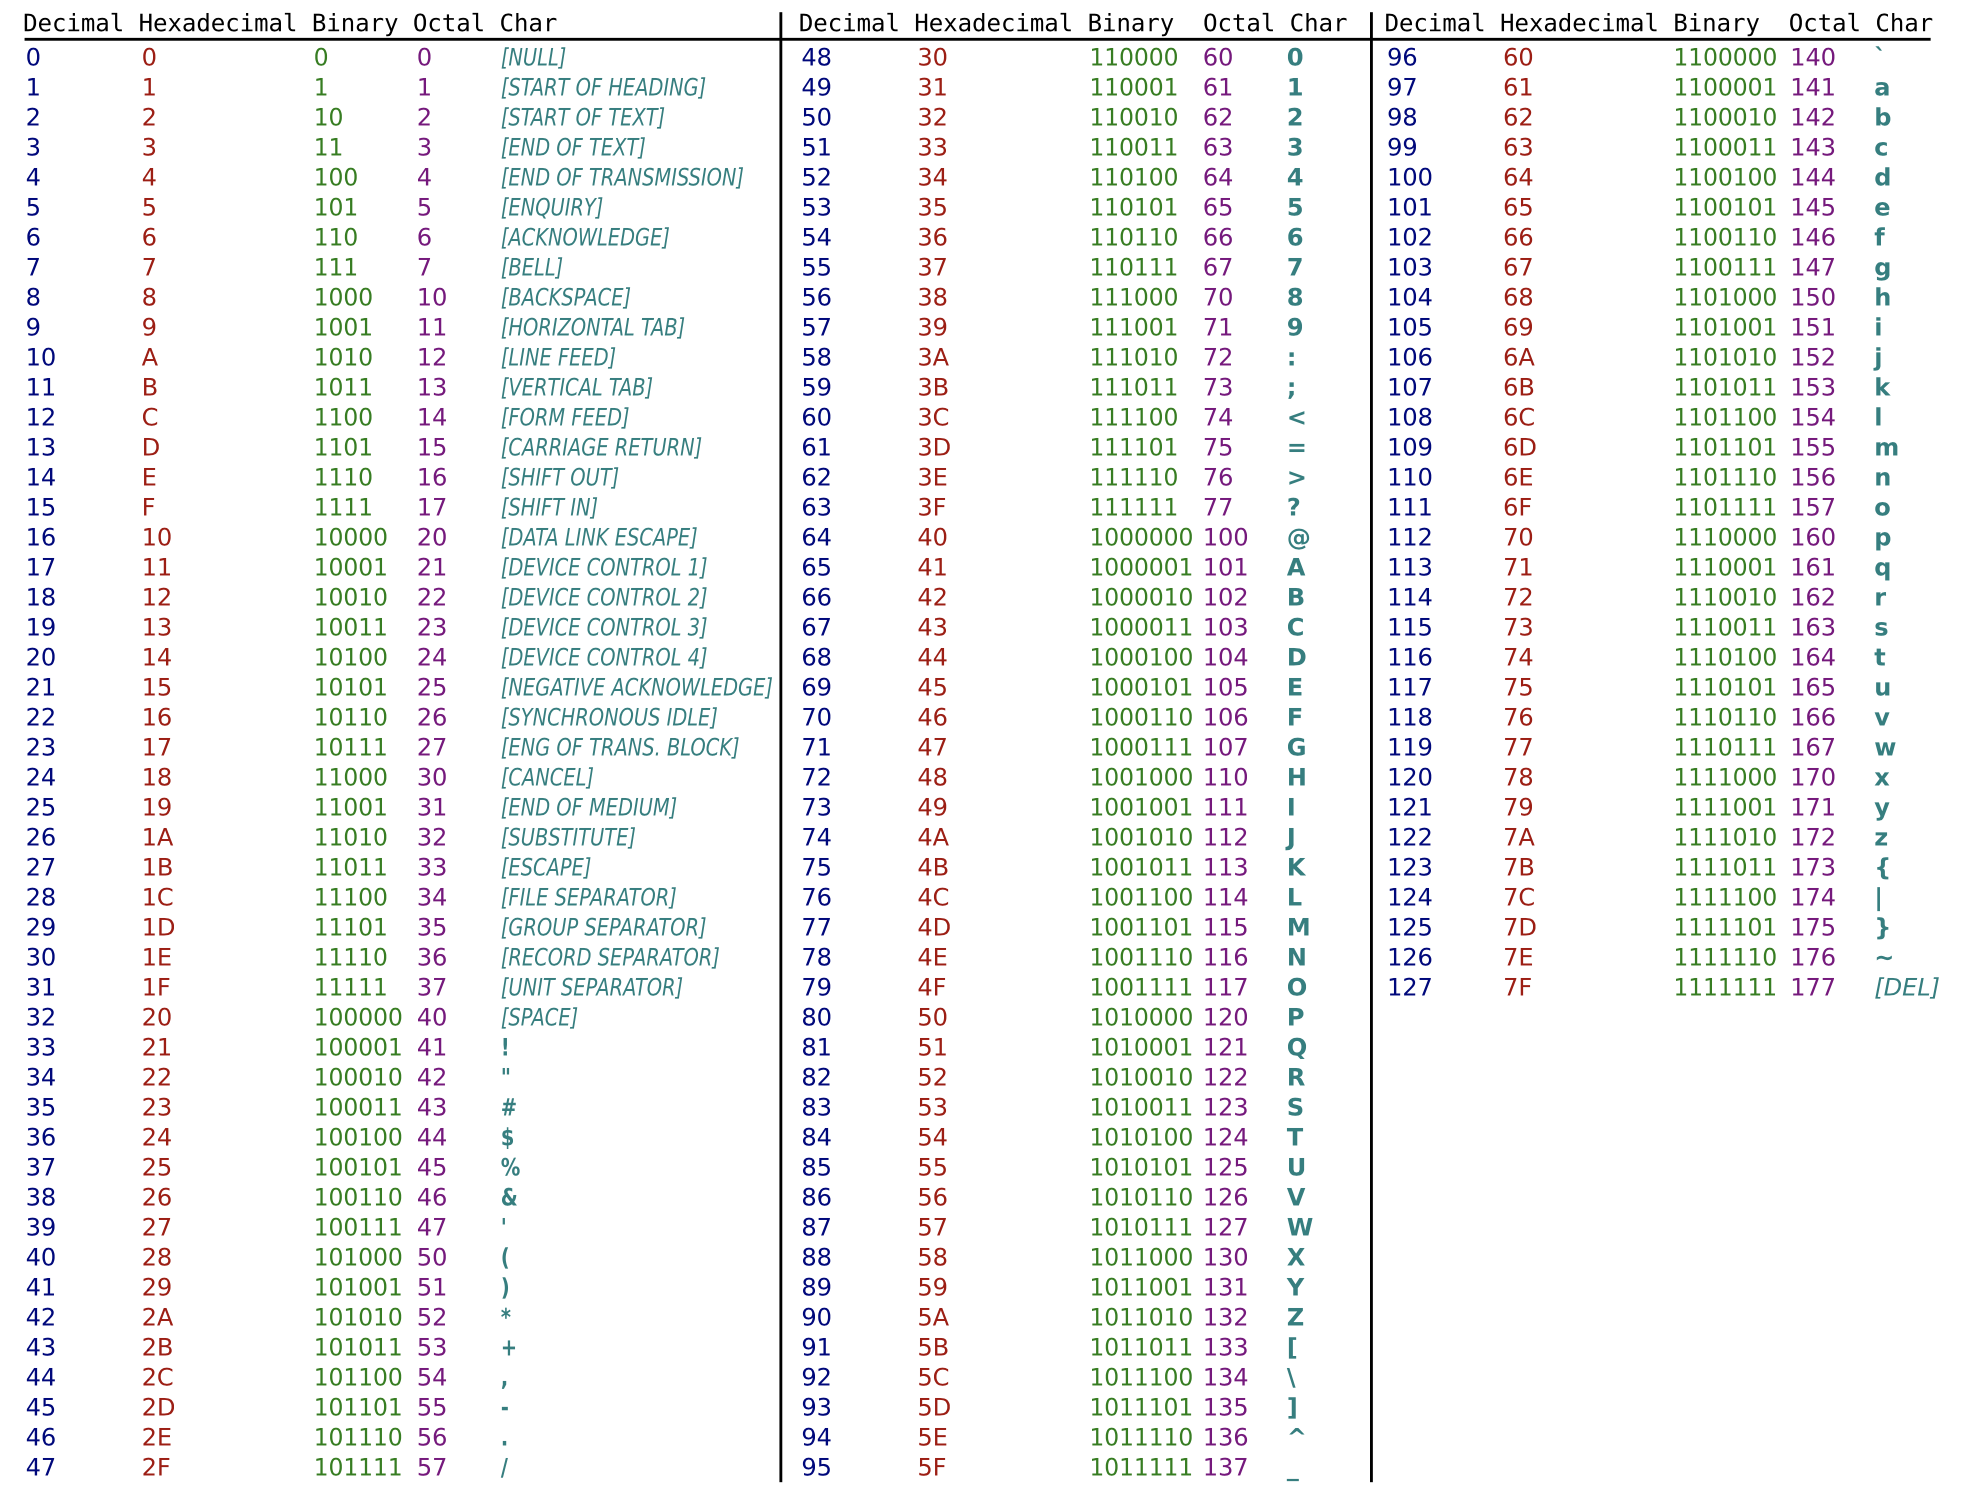
\includegraphics[width=15cm]{ascii}
	\caption{Tablica znaków ASCII}
\end{figure}

\newpage

\section*{\textbf{Fragmenty kodu oprogramowania z wyjaśnieniami} }

\begin{lstlisting}[language=C++, caption=Nakładanie obrazu do kolorowania]
//Funkcja odpowiedzialna za nalozenie na plotno zadanego obrazu
void overlayImage(const cv::Mat &background, const cv::Mat &foreground, 
cv::Mat &output, cv::Point2i location)
{
	background.copyTo(output);
	for(int y = std::max(location.y , 0); y < background.rows; ++y)
	{
		int fY = y - location.y;
		if(fY >= foreground.rows)
		break;
		for(int x = std::max(location.x, 0); x < background.cols; ++x)
		{
			int fX = x - location.x;
			if(fX >= foreground.cols)
			break;
			double opacity =
			((double)foreground.data[fY * foreground.step + fX * foreground.channels() + 3])
			
			/ 255.;
			for(int c = 0; opacity > 0 && c < output.channels(); ++c)
			{
				unsigned char foregroundPx =
				foreground.data[fY * foreground.step + fX * foreground.channels() + c];
				unsigned char backgroundPx =
				background.data[y * background.step + x * background.channels() + c];
				output.data[y*output.step + output.channels()*x + c] =
				backgroundPx * (1.-opacity) + foregroundPx * opacity;
			}
		}
	}
}
\end{lstlisting}

Funkcja overlayImage z argumentami: background, foreground, output i location jest odpo- wiedzialna za nałożenie na przechwycony obraz z kamery durgiej warstwy - w tym wypadku jest to fragment obrazka do pokolorowania (same kontury).
Funkcja w linijce szóstej rozpoczy- na pętle, której zadaniem jest w osiach x i y przychodzących macierzy background i foreground obliczenie i ustawienie w środku generowanego okna obrazu. W linijce 11 zaczyna się sprawdzenie dla osi x po uprzedmim sprawdzeniu osi y. Następnie po ustawniu punktów lokalizacyjnych, w linijce 20 nanoszone są zmiany na ekran poprzez przypisanie mapie nazwie data, która jest elementem zarowno macierzy background jak i foreground.

\newpage




\renewcommand\lstlistlistingname{Fragmenty kodu}
\begin{lstlistoflistings}
\end{lstlistoflistings}


\newpage %każdy punkt główny od nowej linii
\renewcommand\refname{\section*{Bibliografia}}
\begin{thebibliography}{30}\linespread{1}\normalsize{
		%{11} - max liczba źródeł bibliograficznych
		\bibitem{ref1} 
		Wikipedia.org
		\bibitem{ref2}	
		Wybrane dylematy współczesnej edukacji w kontekście "zmediatyzowanej rzeczywistości" - Frania M.
		\bibitem{ref3}	
		Polski Słownik PWN
		\bibitem{ref4}	
		Multimedia w kształceniu - Bednarek J.
		\bibitem{ref5}
		Karol Kuczmarski - Kurs C++. Od zera do gier kodera
		\bibitem{ref6}
		Anders Hejlsberg - The C\# Programming Language
		\bibitem{ref7}
		Christoph Liedtke - Ewolucja grafiki 3D w grach komputerowych
		\bibitem{ref8}
		Ryszard Tadeusiewicz i Przemysław Korohoda - Komputerowa analiza i przetwarzanie obrazów
		
		\bibitem{ref25}
		Nowe media, technologie i trendy w edukacji - Frania M.
		\bibitem{ref26}
		Nowe technologie informacyjne w edukacji - Adamkiewicz J.
		\bibitem{ref27}
		Multimedia w kształceniu - Bednarek J.
		\bibitem{ref28}
		Komputer jako środek dydaktyczny w edukacji wczesnoszkolnej - Hassa A.
		\bibitem{ref29}
		Media w edukacji - Gajda J.
		\bibitem{ref30}
		Słownik terminów i pojęć badań jakościowych nad edukacją - Jagieła J.
	}
\end{thebibliography}

\end{document}
